\documentclass{MScthesisITEM}

% this package is just to generate text for demo-purposes



\title{Village Telco} % The title of your assignement; NB use \newlinetitle to start a newline
\author{Esther Bloemendaal \& Ida Malene Hassel Øveråsen}
\professor{Norvald Stol, ITEM} % Affiliation = ITEM for instance
\supervisor{Sjur Eivind Usken, Lyse Smart AS}

%% Uncomment the following in case you want subfigures; note that there will be a warning for the caption package
% \let\subcaption\undefined
% \let\subfloat\undefined
% \usepackage[bf]{caption}
% \usepackage{subcaption}

\DeclareGraphicsExtensions{.pdf,.jpg}
\graphicspath{{./figs/}}

\loadglsentries{glossary}
\makeglossaries

\begin{document}
\selectlanguage{english}
\pagenumbering{roman}
\pagestyle{plain}

%% Only for the project
\titleITEM

%% Only for the master's thesis; for the project report the description is taken from It's Learning and added by the department
% \selectlanguage{english} % Change to 'norsk' if you are writing in Norwegian
% \begin{titlingpage}

\noindent
\begin{tabular}{@{}p{4cm}l}
\textbf{Title:} 	& \thetitle \\
\textbf{Student:}	& \theauthor \\
\end{tabular}

\vspace{4ex}
\noindent\textbf{Problem description: }
Village Telco is an organization that aims to provide the solution for local communities can deploy data and voice services where no other companies can, or are willing to do so. Village Telco provides a “plug-and-play” solution with low cost voice and data service. While designed for the developing world, Village Telco’s solution can be applied anywhere where people wish to take control of their own telephone infrastructure.

This solution is delivered using an inexpensive fixed mesh WiFi delivery system called the Mesh Potato. The MeshPotato unit is based on the open-source operating system, OpenWRT. Open Source telephony software combined with the latest wireless networking technology creates the potential for people to operate their own community phone systems. Mesh Potato networks have no dependence on existing telecom infrastructure, and can relatively easily be deployed anywhere in the world. It can either be deployed as a stand-alone solution or as an extension to existing technologies. Village Telco’s solution has been deployed in several countries around the world: from East-Timor and Nepal in Asia to several African and South American countries. The installed bases vary from 10 to several hundreds of Mesh Potatoes. 

An area that has not been fully explored is the use of Mesh Potatoes in emergency situations, like natural disasters, post-conflict situations, etc. Another area to be considered is the use of Mesh Potatoes in refugee camps, where many people quickly gather in a new location. In both situations, the need for communication is essential. Key factors of usage are quick roll-out and usability. Easy to use communication is extremely important in crisis situations, both communication within the camp and outgoing communication with the rest of the world. It is important that all affected have easy access to helpful information, as this could mean the difference between life and death in some situations. In refugee camps with thousands of people, registering and reuniting people can be a difficult task to solve. Communication technology, like the Mesh Potato, could be revolutionary in situations like these. 

We will look into how communication is handled by Norwegian emergency relief organizations today, what tools they are using, and if their way of communication could improve with the Mesh Potato. In addition to this, we will look into other existing tools, and explore the possibilities to combine them with the Mesh Potato for a better product.

\vspace{2ex}

\noindent \Blindtext[2][1]
\vspace{6ex}

\noindent
\begin{tabular}{@{}p{4cm}l}
\textbf{Responsible professor:} 	& \theprofessor \\
\textbf{Supervisor:}			& \thesupervisor \\
\end{tabular}

\end{titlingpage}
% \cleardoublepage

%% There must be an abstract in English, even though the main text is in Norwegian
\selectlanguage{english}
\renewcommand{\abstractname}{Abstract}
\begin{abstract}

The Village Telco organization aims to provide affordable communication by means of data and voice services where no other companies are able or willing to do so. Village Telco provides a “plug-and-play” solution with low cost voice and data service. This solution is delivered using an inexpensive fixed mesh WiFi delivery system called Mesh Potato. Village Telco’s solution can be applied anywhere in the world where people wish to take control of their own communications infrastructure. Mesh Potato networks can be deployed either as a stand-alone solution or as an extension to existing technologies. Village Telco’s solution has been deployed in several countries around the world. The installed communities vary from ten, to several hundreds of Mesh Potatoes. 

We directed our studies toward the use of Mesh Potatoes in mobile situations. We have looked at different scenarios covering everything from emergency situations and natural disasters, to festivals and temporary refugee camps. Keith Williamson, a Village Telco volunteer, has created a "go box" using the first generation of the Mesh Potato. We wanted to take his solution further and developed a mobile and stand-alone kit that could be used in all the different scenarios mentioned. The prototype we have developed is slightly different from the "go box". We have used the second generation Mesh Potato and the box includes everything necessary for a quick roll-out; solar panel, battery, different cables and easy to use manuals for configuration. 

We established that many of the descriptions found on the Village Telco wiki were not clear and difficult to use. Hence a big part of our work consisted in simplifying these descriptions. We created manuals for connecting the Mesh Potato to different uplinks in order to provide Internet access to the network. Four test persons, both with and without technical knowledge, tested the manuals. The test process gave us valuable feedback, which led to improvements in the manuals. We have looked at the process of roll-out, and stated possible simplifications and improvements in order to make the roll-out as quick as possible. Hence we have named our solution the \gls{quick} box.

We believe that our work and theoretical research has contributed to and enriched the Village Telco community. Our prototype can be further developed and introduced to relief organizations as well as to others who express an interest in a mobile communications kit. 


\end{abstract}

\cleardoublepage

%% Only for the master's thesis; if the main text is in English and you can write Norwegian, there must be an abstract in Norwegian as well.A
% \selectlanguage{norsk}
% \renewcommand{\abstractname}{Abstract}
\begin{abstract}


* Hvorfor vi gjør det som vi gjør, hva er bakgrunnen

* Hva har vi gjort

* hvordan har vi gjort det

* hva fant vi ut

* hva resulterer det i hva konkluderer vi med?



Village Telco is an organization that aims to provide affordable communication in forms of data and voice services where no other companies can, or are willing to do so. Village Telco provides a “plug-and-play” solution with low cost voice and data service. While designed for the developing world, Village Telco’s solution can be applied anywhere people wish to take control of their own communication infrastructure.

This solution is delivered using an inexpensive fixed mesh WiFi delivery system called the Mesh Potato. The Mesh Potato unit is based on the open-source operating system, OpenWRT. Open Source telephony software combined with the latest wireless networking technology creates the potential for people to operate their own community phone systems. Mesh Potato networks have no dependence on existing telecom infrastructure, and can relatively easily be deployed anywhere in the world. It can either be deployed as a stand-alone solution or as an extension to existing technologies. Village Telco’s solution has been deployed in several countries around the world: from East-Timor and Nepal in Asia to several African and South America countries. The installed bases vary from 10 to several hundreds of Mesh Potatoes. 

We have directed our studies toward the use of Mesh Potatoes in mobile situations. We started by looking into different scenarios consisting of everything from emergency situations and natural disasters, to festivals and temporary refugee camps. After being in contact with different relief organization we got a clear impression that communication under and after a disaster situation is a difficult task. Keith Williamson, a Village Telco volunteer, has created a "go box" using the first generation of the Mesh Potato. We wanted to take his solution further and develop a mobile and stand-alone kit that could be used in all the different scenarios that we have taken into consideration. The prototype we developed differs from the one already made. We have used the second generation Mesh Potato and the box includes everything necessary, solar panel, battery, different cables and easy to use manuals for configuration. 

In the process of creating this kit we had to set up the network in order to conduct testing, both of the network and the configurations. We found that many of the descriptions found on the Village Telco wiki were little explanatory and difficult to use. Therefore a big part of our work has been to simplify these descriptions, and make them easy that little or non-technical people can use and understand them. We have looked at simplifications as well as processes in order to make the roll-out as quick as possible. Hence we have named our solution the \gls{quick} box.

* Fylle ut mer her etter at vi har skrevet konklusjonen

We believe that our work and theoretical research has contributed and richened Village Telco. And eventually save lives. 






\end{abstract}
% \cleardoublepage

\selectlanguage{english}% Change to 'norsk' if you are writing in Norwegian

\renewcommand{\abstractname}{Preface}
\begin{abstract}

This study was performed as a master's thesis on behalf of the \gls{item} at the \gls{ntnu}, in cooperation with Village Telco. This report is the final result of this master's thesis and is worth 30 ECTS points. The study was conducted between January and June 2014. The project description was outlined in cooperation with our project supervisor Sjur Usken from Aarbakke Innovation AS.

We would like to thank Sjur Eivind Usken who has guided us throughout our project, and contributed with helpful ideas, feedback and support. We would also like to thank our project professor Norvald Stol for his helpful feedback and support. We thank the Village Telco community, especially Steve Song and Keith Williamson, for taking the time to answer our questions and for helping us along the way. Also a thanks to Marte Berg Innset for the collaboration on the background chapter. Finally, we would like to thank everyone who helped us test the prototype of the QUICK box. \\

\vspace*{2\baselineskip}
\paragraph{}
Trondheim, June 11, 2014
\vspace*{1.5\baselineskip}
\paragraph{}
Esther Bloemendaal
\paragraph{}
Ida Malene Hassel Øveråsen


\end{abstract}
\cleardoublepage

% similarly you may add a separate acknowledgments page

\tableofcontents*
\cleardoublepage

%% include if relevant
\listoffigures
\cleardoublepage

%% include if relevant
\listoftables
\cleardoublepage

%% include if relevant
\listofalgorithms
\addcontentsline{toc}{chapter}{List of Algorithms}
\cleardoublepage

%% include if relevant
\printglossary[title=List of Symbols, style=long]
\cleardoublepage
\glsaddall[]

%% include if relevant
\printglossary[title=List of Acronyms,type=\acronymtype] % prints just the list of acronyms
\cleardoublepage

\pagenumbering{arabic}
\pagestyle{ruled}

\chapter{Introduction}
\label{chp:introduction} 
%% include here the other chapters

\chapter{Background}
\label{chp:background} 

\section{Village Telco}
%How did it all start?

\section{Mesh Potato}
%Generelt om MP

% hvordan MPen fikk navnet. 


%MP01
<<<<<<< HEAD
The whole concept around the Mesh Potato was developed in June 2008 during a workshop with the Village Telco team. The aim was to develop a business model as well as a prototype for a Villa Telco. Initially the idea was to use low cost VoIP headsets. At the time this was the most viable and convenient way to deliver telephone services to the customers. With a VoIP telephone service the nodes can not be more that 100 meters away from each other, requiring more nodes to be able to cover the desirable area. Which again drastically increases the start-up costs for a village. In order to keep the cost down, it was also important to keep the number of access points down. A mesh network have a larger range, and one suggestion was to use a small mesh device like a Open Mesh AP and connect a SIP phone to it. This solution would solve a lot of the problems regarding range, antenna and number of access points, but the idea was still an expensive option. During the debating, Rael Lissoos took a Analouge Telephone Adapter (ATA) and an Open Mesh AP, held them together and said that we need these two devices in one. This point was the birth of the Mesh Potato. The name comes from combining the words mesh, POTS (Plain Old Telephone) and ATA. Patata is the Spanish word for potato, and hence the name Mesh Potato. A mesh enabled WiFi device with the possibility to connect any inexpensive regular phone and IP device. \cite{MPorigin}
=======
The whole concept around the Mesh Potato was developed in June 2008 during a workshop with the Village Telco team. The aim was to develop a business model as well as a prototype for a Village Telco. Initially the idea was to use low cost VoIP headsets since it was the most viable and convenient way to deliver telephone services to the customers. With a VoIP telephone service the nodes can not be more than 100 meters away from each other requiring more nodes to be able to cover the desirable area. Which again drastically increased the start-up costs for a village. In order to keep the cost down, it is also important to keep the number of access points down. A mesh network have a larger range, and one suggestion was to use a small mesh device like a Open Mesh AP and connect a SIP phone to it. This solution would solve a lot of the problems regarding range, antenna and number of access points, but the idea was still an expensive option. During the debating, Rael Lissoos took a Analouge Telephone Adapter (ATA) and an Open Mesh AP, held them together and said that we need these two devices in one. This point was the birth of the Mesh Potato. The name comes from combining the words mesh, POTS (Plain Old Telephone) and ATA. "Patata" is the Spanish word for potato, and hence the name Mesh Potato. A mesh enabled WiFi device with the possibility to connect any inexpensive regular phone and IP device. \cite{MPorigin}
>>>>>>> 48118eeb54d92f9fb9eb7897a927417878f85a17

\begin{figure}[h!]
  \centering
      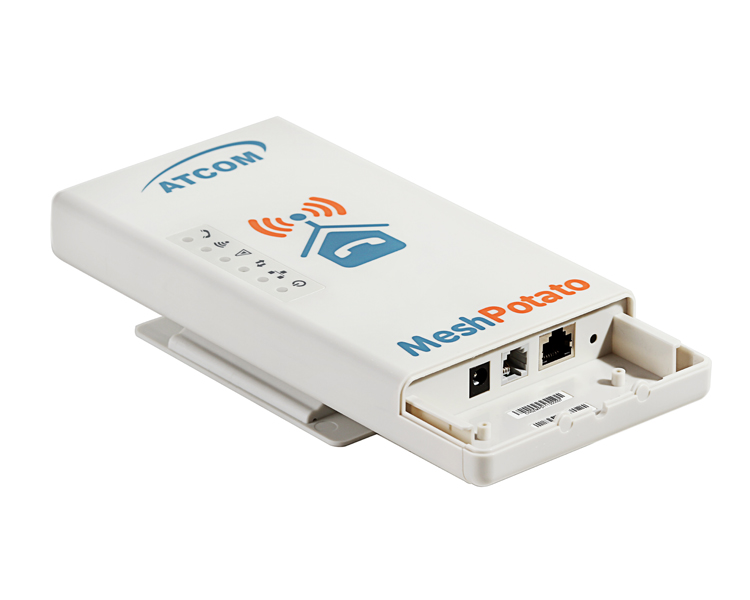
\includegraphics[width=0.5\textwidth]{MP01}
  \caption [The Mesh Potato]{\textbf{The fist generation Mesh Potato, MP01}}
  \label{fig:MP01}
\end{figure}

The First generation of the Mesh Potato is shown in \fref{fig:MP01}. This device is designed to be used in rural areas. It can be deployed and run anywhere in the world relying only on a low, but stable power supply. The Ethernet port, Foreign eXchange Station (FXS) ports and power are robust and designed. This in order to handle hard weather, poor power conditions, lightening and static electricity. In addition the Mesh Potato comes in a waterproof box for outdoor mounting \cite{background}.

The Mesh Potato combines the features of a 802.11bg WiFi router with an Analog telephone Adaptor (ATA) \cite{MP}. Each Mesh Potato provides a single fixed telephone line to the end user. The MPs are connected together via a mesh WiFi network, and  configure themselves automatically to form a peer-to-peer network, greatly extending the range of the network over regular WiFi. Enabling phone calls to be made independent of landlines and telephone towers. Creating the basis for the "plug-and-play" solution. 








The Mesh network can be connected via backbone link to the rest of the world by using VoIP trunks. 


MP02





\section{Technology}

\subsection{Ad Hoc and Mesh Networks}

\begin{figure}[h!]
  \centering
    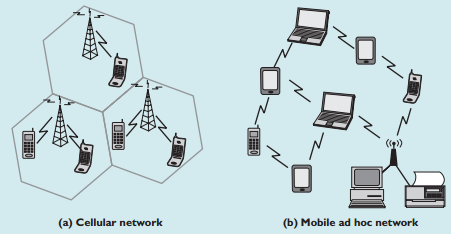
\includegraphics[width=0.8\textwidth]{adhoc.png}
     \caption [Cellular network vs. MANET]{\textbf{Cellular network vs. MANET}. This figure illustrates the difference between a regular cellular network and a mobile ad hoc network \cite{adhoc2}.}
\label{fig:adhoc}
\end{figure}

\subsubsection{MANETs} Mobile ad hoc networks (MANETs) are networks that does not rely on an underlying and fixed infrastructure (access points and routers), in other words infrastructureless. MANETs acts in a shared wireless media \cite{adhoc}. The structure of these networks change dynamically, and key factors for MANETs is self-configuration and self-organization. The members of the network are mobile and are free to join or leave the network \cite{adhoc2}, and therefore these factors are important. MANETs are based on multi-hop forwarding. This means that each node acts not only as a host, but also as a router. The nodes themselves establishes and maintain routes, and forward packets to other nodes if necessary. This enables communication between nodes that are originally not within each other's send range \cite{adhoc2}. Because of these characteristics MANETs is suited for use in situations where there are no fixed underlying infrastructure. MANETs can operate as a stand-alone solution, but it can also be attached to the Internet. This makes room for numerous of services. 

\begin{figure}[h!]
  \centering
    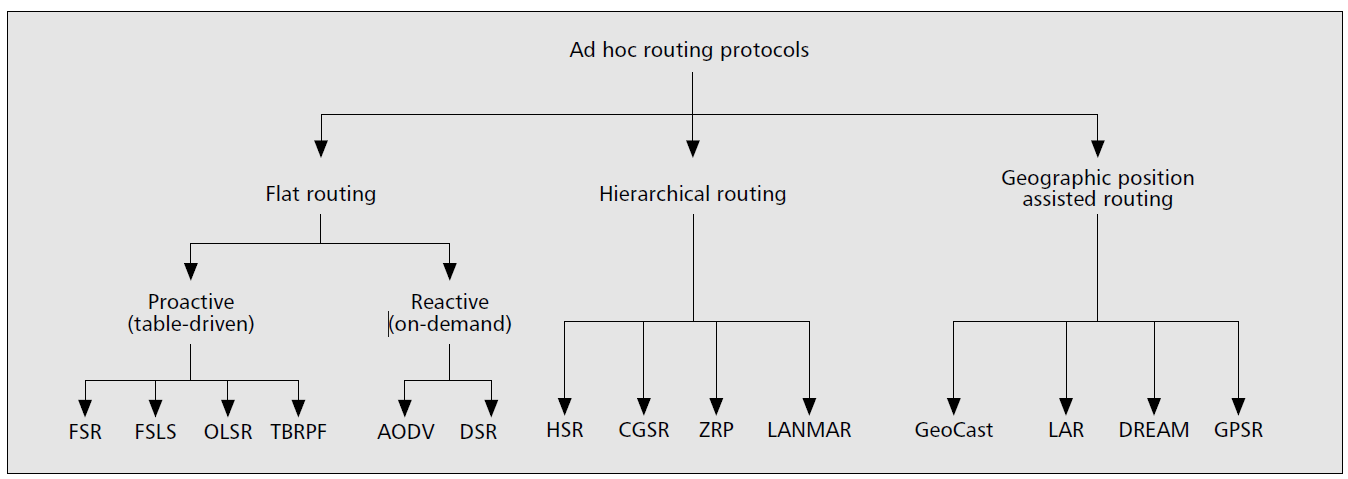
\includegraphics[width=1\textwidth]{adhocprotocols.png}
     \caption{Different groups of ad hoc routing protocols \cite{adhoc}.}
\label{fig:adhocprotocols}
\end{figure}


\subsubsection{Routing Protocols}
There exists many challenges when it comes to these types of networks. The routing protocols must be able to adapt quickly due to the topology changes. \fref{fig:adhocprotocols} shows the different groups of the ad hoc protocols that exist. The routing protocols must not cause excessive overhead. Under the category flat routing, there are two types of routing protocols; proactive and reactive. \textit{Proactive routing protocols} (e.g. OLSR) are table driven \citep{proactivereactive}. This means that every network node has a routing table for the forwarding of data. To obtain stability, each node broadcasts and modifies the routing table periodically. Proactive routing protocols are suitable when there are few nodes in the network. Because of the routing table that is periodically updated, the overhead exceeds the desired value when there are a high number of nodes in the network. In contrary to the proactive routing protocols, \textit{reactive routing protocols} (e.g. AODV) are on demand. Since they are on demand, the overhead is significantly lower. These protocols utilizes flooding. The network is flooded with the route request (RREQ) in order to set up the route. The reactive routing protocols does not have a up-to-date routing table like proactive routing protocols \cite{proactivereactive}. Routes are only set up to nodes they communicate with, and these routes are only kept alive while they are needed  \cite{adhoc2}. As shown in \fref{fig:adhocprotocols}, there are several different protocols under proactive and reactive. 

\paragraph{B.A.T.M.A.N}
Better Approach To Mobile Adhoc Networking (B.A.T.M.A.N) is the routing protocol utilized in the networks formed by the Mesh Potatoes. B.A.T.M.A.N is a proactive routing protocol for wireless ad hoc networks. This includes MANETs \cite{batman}. This protocol was developed as an alternative to OLSR (Optimized Link State Routing) \cite{batman2}. Like mentioned before, routing protocols must be able to adapt quickly to topology changes. B.A.T.M.A.N was made to be a more efficient routing protocol in this area. 

Information about the nodes that are accessible via single-hop or multi-hop are maintained and updated. 


%Eksempel på nettverk

\subsection{OpenWrt}

\section{The Cost Structure and Revenue Model(s) of Village Telco Today}

\section{Comparison of Village Telco and Other Telcos}

\section{Refugee Camps}
\subsection{The Existing Communication Methods}
\chapter{Refugee Camps}
\label{chp:refugeecamps} 

\section{Refugee Camps}
%Generell fakta

Women are in general in a more vulnerable position when living in a  camp, especially if they are single mothers. They may be solely responsible for taking care of the children in addition to sick and elderly family members, maintaining the household, preparing food, acquire water, and securing firewood. Collecting firewood for cooking is a necessity, but it forces women  to walk far away, hence making them vulnerable for sexual assault. they have to turn to sex and other unhealthy and dangerous means in order to survive. \cite{womenRefugee} 


The means of communication vary greatly in the different camps. Some have internet connection and satellite TV, other barely have access to a radio. Even though radios are the most common media for communication, it is not given that all citizens in a camp have access to one. Often people would gather around the few radios that exists in a camp. One issue that limits the usage is the batteries. They are very expensive and hard to acquire. The women were interested in news regarding their place of origin. 

Information walls and word of mouth is often used in order to spread practical information within the camp and about camp activities. Word of mouth is also used in order to retrieve information about the world outside the camp. People visiting the camp were used as sources for information. Earlier studies have shown that social connections with neighbours works as an important medium to transport information, resources and services between individuals. These kind of networking have been used to find lost family members in big camps, as well as get financial help from abroad \cite{womenRefugee}.  



\paragraph{Cell Phone}
The use of cell phones are increasing. Even though the prises are extremely high it does not stop people from calling relatives in Europe and other places in the world. 
\cite{womenRefugee} 


\section{Statistics}
When we talk about refugees it is important to divide between different types of refugees, mainly a refugee and an IDP. 

\paragraph{Refugee.} The definition of a refugee is a person who have been forced to leave their home country because of war, violence or persecution. A refugee often has a justifiable fear of persecution for reasons as religion, political opinion, race, nationality or membership in a certain social group. For these reasons are not able to, or are afraid to  return to their home country. The leading reasons for refugees flee their home country is war and ethnic, religious and tribal violence \cite{refugeeDef}.

\paragraph{Internally Displaced Person.} An internally displaced person (IDP) is a person that has been forced to leave their home and village for some reason and are a refugee in its own country. The man distinction between an IDP and a refugee is that the person has not crossed any country borders. Unlike refugees, the IDPs are not protected by any international laws nor are able to receive many types aids. in the last years the number of IDPs have drastically increased, mostly due to the conflicts between countries. 

A stateless person is someone who does not have citizenship in any country. a citizenship is a legal bond between an individual and the government in that country. 

By the end of 2012 45.2 million people were displaced by force. According to UNHCR is this the largest number in 20 years. The report show that 55 \% of the registered refugees came from countries affected by war as Syria, Afghanistan, Sudan, Iraq and Somalia. The crisis in Syria has been a major factor to displacement, the whole of 647,000 people have be forced out of the country \citep{UNHCRstat}.

In 2012 UNHCR registered 21,300 individual asylum applications from children that either were unaccompanied or separated from their family. 


\section{Interview with CARE - Dadaab Refugee Camp}
We got in contact with Mary Muia from CARE. She is a program assistant at CARE International in Dadaab, Kenya. We sent her a questionnaire with questions about Dadaab refugee camp, with focus on means of communication. The following paragraphs contains information both from different articles referred to in the text, and from the questionnaire. See Appendix \ref{chp:appendixA} for the full questionnaire. Dadaab is the largest refugee camp in the world, and is located in Daadaab, Kenya \cite{dadaab}. It was created in 1991 \cite{dadaabcare}. Dadaab was created by the government of Kenya and UNHCR to host Somali refugees displaced by civil war. Over the years, the camps have also hosted other nationalities, from the Horn of Africa, the Great Lakes and East Africa regions. These people constitute less than two percent of the camp population. In April, 2013, there were 423,496 registered refugees in the Dadaab camps. 51 \% of these were female and 58 \% were younger than 18 years old. Also in 2013, UNHCR and its partners decided to conduct a verification exercise to ascertain the current population. The reason for this was that many of those who had arrived in 2011 due to the famile had returned home. As at February, 2014, the current population stands at 369,294. The lead agency for this camp is the UN High Commission for Refugees (UNHCR) \cite{dadaab}. In addition to UNHCR, major international humanitarian agencies like Care, Save the Children and the International Rescue Committee  are active helpers in the Dadaab refugee camp. These agencies provide the refugees with critical services (e.g. food, housing, sanitation and medical help). This is an extremely challenging task in refugee camps, especially when they reach this size. During the recent years, the terror group Al Shabaad (Somali-based) have intensified their misdeeds in and around the Dadaab refugee camps. This has made the situation even tougher for the refugees and the relief agencies. 
Muia states that the biggest challenges in the camps are lack of enough space to accommodate everyone, and lack of enough funds to take care of alle the needs of the refugees. Another challenge is the language barrier between the humanitarian staff and the refugees. Many of the staff members do neither speak nor understand the Somali language, and as many as 95.6\% of the refugees are Somali. 


Muia explains how the registration process is handled. When a new refugee enters the camp, the refugee reports to a UNHCR reception desk. There the refugee is given a temporary registration, while pending full registration. Upon arrival, the refugees are given information about available services, and which agency is handling what service. Immunizations, medical attention, emergency food supply, tarpaulins, sleeping mats, jerrycans for fetching water and kitchen sets are issued to new arrivals. This is to help them start their new lives in the camp. 

To improve the situation in Dadaab, communication is crucial. In 2011, a group consisting of people from NetHope, Inveneo and the USAID Global Broadband and Innovations Program gathered to discuss ways to improve the means of communication in Dadaab \cite{dadaab}. NetHope is a consortium of over 30 international Non-Governmental Organizations (NGOs) \cite{nethope}. NetHope works with improving connectivity, with the help of information technology, among relief agencies. The aim of this project, called DadaabConnect, was to bring forward more reliable Internet, and find ways for agencies to communicate better internally \cite{dadaab}. The group put together teams that travelled to Kenya to investigate the conditions in the refugee camps, and to find out what they could implement. It was clear from the feedback they got that a better communication system was needed, and that it would make the humanitarian work much easier. It would improve the coordination and the security in the camps. Improvements of these aspects gives the humanitarian agencies better working conditions, and makes it easier for them to help the refugees with critical services. Inveneo started working with Cisco's Tactical Operations (TacOps) to install and configure a local high-speed network \cite{dadaabinveneo}. They also entered a partnership with a local Kenyan mobile and landline telecommunications service provider called Orange. The reason for this was that they wanted to extend the Dadaab compound with new data services. This could be done by using Inveneo's long-distance Wi-Fi solutions. The data services that were added included services requested from the Dadaab aid community. "DadaabNet", a high-speed network, was created in cooperation between Inveneo and TacOps. This network connected the NGOs locally, and made it possible for the agencies to easier communicate internally (VoIP telephony, file sharing etc.). Following this, in March 2012, they started the training of technicians. These technicians were people from Orange, from the technical staff of the NGOs and from Inveneo's staff. The training took place both in classrooms and in the field, in order to give the technicians a wide understanding. The results from DadaabConnect has been great. The humanitarian agencies has gotten better working conditions, due to the improvements in means of communication. Other positive outcomes is that the network is more reliable and cost effective. 

Muia did not specifically mention this project in her answers, but answers on our questions about means of communication within the camp, and with the outside world. She states that CARE as an organization has invested in communication systems in cooperation with ISPs in the capital city of Kenya, Nairobi. Through this cooperation the camp staff are assured to get access to Internet for both official and social use. Several Kenyan telecommunication companies have put up equipment in the camp area, and the camps are therefore provided with access to mobile communication and Internet. Although this is set up, Internet and telephone service outages are fairly common. In addition to mobile communication and Internet, there are radio station services and access to digital television. CARE use telephone services to reach out to refugee staff. 50\% of the refugees have access to mobile phone services. Posters an radio is also used to reach out. Word by mouth (e.g. over speakers) is also a communication technique employed. There are two main telecommunication providers in Dadaad, hence little competition. This makes the prices higher. We asked Muia how the refugees can afford having their own mobile phone, when the costs are high. She says that many refugees have been in the camps for a long time, and therefore have had the time to establish small businesses which gives them some profit. While others get money sent from their relatives. 


\section{Interview with Norwegian Refugee Council}
%hun mener vi skal klassifiere for oppgaven sin del av vi snakker om offisielle leirer. UNHCR har ansvar da. Monitirere enklere da om de tingene er på plass, og evt. hva slags system de bruker. 

We had a Skype interview March 12, 2014, with Katrine Wold from the Norwegian Refugee Council (NRC). The aim of the interview was to hear a little bit about her work in refugee camps and how the situation in the refugee camps are today, with main focus on means of communication.
Katrine Wold has been working for NRC for many years, and also has a background from United Nations (UN). She has worked in emergency and crisis situations abroad. She is specialized in camp management and coordination. In recent years she has been responsible for education, and have had the main focus on youth. We asked her which refugee camps NRC is working in, but she could not give us a clear answer on that question. The reason for this is that NRC works in over 24 countries, and have, as of 2013, reached out to 4.4 million people. She makes it clear that there are a difference between internally displaced persons (IDPs) and refugees. An official refugee must cross a boarder, or else you are internally displaced. NRC works both with refugees and IDPs, and also with people who are affected by having refugees in their local area. NRC does not only help with operational issues in the camps, but they mainly offer services the refugees need. When dealing with refugees there exists international laws and regulations. These also states what kind of human rights exists. Everyone have rights! The vast majority of countries have ratified the UN refugee commission, which has been formed by the international society, UN, and authorities via UN's forums. The commission is an important premise when working with refugees. It is important to know which rights you have as a humanitarian worker, and which rights the refugees have. 

We ask her about how communication within the camp is conducted. She takes Kenya as an example. NRC has been working in the largest refugee camp in the world, Dadaab Kenya, for many years.  Some have the main responsibility for what is going on in the camp, and that is the  authorities. They often ask the international community (e.g. NRC) for help. Wold states that it is then important to establish good communication and information flow between the ones working in the camp (the different organizations). This communication takes places by either establishing coordination meetings and by other types of mechanisms. These meetings includes the relief organizations working in the camp, and the authorities. The goal is not to make a permanent home for the refugees, but that it is safe when they are in the camps and that they move on (either go home or find another place to live). Living in camps is a temporary life situation. She states the different types of communication; internally between the workers in the camp and communication with the refugees. It is important to establish open transparent coordination mechanisms, in other words ensure good forums where the refugees can communicate and inform the workers in the camp what their needs are. This can only be achieved by recognizing that refugees is not a large mass, but individuals with different needs and different life situations. The humanitarian and authorities try to establish some sort of local elections. This means that the refugees can choose representatives who's job is to be in communication with the primary humanitarian managers in the camp. The reason for this is that it is impossible for the humanitarians to talk to 500 000 people. The communication between the representatives and the managers be done either through meetings, or in an informal manner. Overall, this creates a communication pattern in the refugee camps. Wold states that there a few places without mobile coverage, and that the majority of the refugees have a mobile phone. Mobile phones are used frequently in terms of distribution. Mobile phones are often used as a tool when goods (access to money, food etc.) gets distributed to the refugees. They can "add credit" to their card, and use this as "payment". This an up-and-coming way of doing distribution. Mobile phones are also used to collect information, for example by sending the refugees surveys on their mobile phone. 


In general, Wold states that methods of communication can be via mouth, radio, billboards, data communication, but this all depends on which camp and what is allowed in the camp. The law in the refugee camps depends on the national authorities. In some camps it is allowed to establish a data communication center, but in other camps this is illegal. It is important that when the refugees arrive to a camp that they get informed of the current situation, and what rights they have. The distribution of this information takes places primary by someone called the camp management agency. They have the daily coordination responsibility for what is going to take place in the camp. It must be made clear to the refugees where they can obtain different types of services, and also what is expected of the refugees. It is important that the refugees at an early stage get the opportunity to contribute positively in the camp, or else they can end up with something called "dependency syndrome" (they feel incompetent and get totally dependent on external assistance). 

Another question we asked her is how the refugees get registered in the camps. Here she states the importance of distinguishing between official and unofficial camps. The definition of a camp is that people are gathered together and live there. Registration is done in official camps, and then there are someone who is responsible for the operation of the camp. When refugees are registered they get an ID card. This ID card is very valuable, because it indicates that you, as a refugee, have access to the goods that are available in the camp. The registration procedures can vary, but most often there exists computer systems for the registration.




\renewcommand*{\bibname}{References}
\bibliographystyle{ieeetr}
\bibliography{references}

\appendix
\addtocontents{toc}{
	\protect\vspace{1em}
	\protect\noindent \bfseries \appendixtocname\protect\par
	\protect\vspace{-.5em}
}
\renewcommand{\chaptername}{\appendixname}
%\chapter{Interview with Care}
\label{chp:appendixA} 

This appendix contains the summary from the interview conducted on Mary Muia (CARE International in Kenya | Program Assistant
Refugee Assistance Programme | Dadaab).


\begin{enumerate}

\item Approximately how many people are there in the Dadaab refugee camp? And how long have it been in operation?

The Dadaab complex of refugee camps, considered the world’s largest, was created in 1991 by the Government of Kenya and UNHCR to host Somali refugees displaced by civil war. Over the years, the camps have also hosted other nationalities from the Horn of Africa, the Great Lakes and East Africa regions but they constitute less than two percent of the camp population. The original camps were Dagahaley, Ifo and Hagadera and were intended to host 90,000 refugees. However, in 2011, there was an influx of new refugees from Somalia due to severe drought and new camps were created; Ifo 2 and Kambioos, to cater to the over 175,000 new arrivals and at the peak of the influx in 2011, the camps hosted more than 463,000 refugees, including some 10,000 third-generation refugees born in Dadaab to refugee parents who were also born there. However, in 2013, UNHCR and its partners conducted a verification exercise to ascertain the current population since some of those who had arrived in 2011 due to the famine had returned home. As at February, 2014, the current population stands at 369,294.

\item How do you connect and communicate with the outside world?

CARE as an organization has invested in communication systems in liaison with Internet Service Providers in the capital city of Nairobi who ensure that all staff have access to internet for both official and social usage.

\item How are the communication inside the camp (communication flow)?

Several telecommunication firms in Kenya have put up their machinery in the area thus there is access to both mobile communication and access to internet services. There are also radio station services and access to digital televisions. CARE uses telephone services to reach out to refugee staff (50\%) of the refugees have access to mobile phone services - either owned or through a bureau) posters and radio to reach out to its beneficiary population. In addition, there is word of mouth done through loud speakers during major gatherings like food distribution days and also road shows within the camps.


\item How does the refugees receive information?

As 3 above.

\item Can you exlain what happens when a new person enters the camp?

Upon arrival, a new refugee would report to a UNHCR reception desk whereby they are given temporary registration pending full registration and location of their relatives is they have any already in the camp. UNHCR fully briefs the new arrival on all the services available and which Agency is handling what service. Immunizations, medical attention, emergency food supply, tarpaulins, sleeping mats, jerrycans for fetching water and kitchen sets are issued to such new arrivals to help them start their new lives in the camps. UNHCR then hands over the new arrivals to the respective Agency doing camp management in the specific camp they are allocated so that they can be shown where to pitch their tents. The camps are well demarcated into numbered sections and blocks thus at any given time, UNHCR would inform you where a particular refugee resides and the family size. Each Agency working in Dadaab has their own mode of communicating the services they provide to their target beneficiaries. However, UNHCR holds regular meetings with the refugee leaders of each respective camp whereby information is shared with them for dissemination to the entire refugee population.


\item What are the biggest challenges in a refugee camp?

Lack of enough space to accommodate everyone and lack of enough funds to take care of all the needs of the refugees.


\item What is the biggest challenge when it comes to communication/information spreading in the refugee camp?

Language barrier between the humanitarian staff and the refugees since many of the staff do not speak/understand the Somali language while 95.6\% of the refugees are Somali. Internet and telephone service outages are also common in the area and response by the service providers sometime take a while.


\item What means of communication do you use in the refugee camp?

Mobile phones and computers for both telephone and internet access. Radios and television services.


\item How long does it take to set up a communication system?

N/A since I am not a technical person


\item Do you use video surveillance?

No

\item Have you heard of something called Freedom fone?

No

\item Have you heard of the company Village Telco?

No


\item Do you have anything else to add that can be of interest for our master thesis?

No

\end{enumerate}
%\chapter{SECN-1.1 User Guide}
\label{chp:appendixB} 


\includepdf[pages={1-38}]{SECN.pdf}


\end{document} 
